\title{60-371\\Artificial Intelligence\\Iterated Prisoner's Dilemma}
\author{
		Quinn Perfetto \\
        William Roeder \\
        David Valleau
}
\date{\today}

\documentclass[12pt]{article}

\usepackage{ amssymb }
\usepackage{longtable}
\usepackage[T1]{fontenc}
\usepackage{tocloft}
\usepackage{hyperref}
\usepackage[none]{hyphenat}
\usepackage[]{algorithm2e}
\usepackage{graphicx}
\hypersetup{
    colorlinks=true,
    linkcolor=black,
    urlcolor=blue
}
\renewcommand\cftsecleader{\cftdotfill{\cftdotsep}}
\setlength\parindent{0pt}

\SetKwInput{KwInput}{Input}
\SetKwInput{KwOutput}{Output}

\begin{document}
\maketitle

\pagebreak
\tableofcontents
\pagebreak

\section{Abstract}

This paper explores the use of two Artificial Intelligence algorithms to
create optimal strategies to compete in the Iterated Prisoner's Dilemma.  The
study begins by examining the use of a genetic algorithm to breed the perfect
prisoner.  Several different configurations and fitness functions were tested and
the performance of each was contrasted.  The genetic algorithm was able to
consistently breed well performing prisoners.
A hill climbing approach was then taken,
which proved to be ineffective at producing a competitive strategy given the
lack of a natural successor function and no clear end goal.  Finally, the traits
of a "good" genome are explored and the performance of the two methods are contrasted.

\pagebreak

\section{Introduction}
The Iterated Prisoner's Dilemma is a classic example of game theory which demonstrates
that two agents acting for their own self interest may not result in an
optimal outcome for either agent.  The prisoner's
dilemma is as follows: \\ \\
Two individuals (herein Bob and Alice) have been arrested and placed in solitary
confinement so that they may not communicate with one another.  Each of them hope
to spend the least amount of time in prison.  The prosecutor approaches them
and offers the following deal:
\begin{itemize}
    \item If Bob and Alice betray (herein defect) each other, they will
        both serve 2 years in prison
    \item If Bob defects but Alice remains silent (herein cooperate), Bob
        will be set free and Alice will spend 3 years in prison (and vice versa)
    \item If Bob and Alice both cooperate they will each spend 1 year in prison
        on a lesser charge \\
\end{itemize}

The iterated version of the prisoner's dilemma is simply a sequence of rounds of
the above mentioned game.  A player's score is the summation of their score in
each round. \\

It is implied that Bob and Alice will have no interactions with each other after
their decisions and thus cannot punish/reward their accomplice. If Bob and Alice are
both rational and self centered then they will both choose to defect, as defecting
yields the highest probability of a favourable outcome.  It is interesting to note
that if the prisoners act non-rationally and choose to cooperate
(the "riskier" option) they will spend 1/3 of the time in prison compared
to the rational option. \\

Taking after J. Golbeck
\footnote{\href{http://cgis.cs.umd.edu/~golbeck/downloads/JGolbeck\_prison.pdf}
{Evolving Strategies for the Prisoner's Dilemma}}
the payoff matrix for this study has been
inverted such that a higher score implies a lesser sentence. \\

\begin{center}
    \begin{tabular}{l | c | c}
         & Cooperate & Defect \\
        \hline
        Cooperate & (3,3) & (5, 0)\\
        \hline
        Defect & (0, 5) & (1,1) \\ \\
    \end{tabular}
\end{center}

Iterated prisoner's dilemma strategies have been widely studied, and many have
concluded that Tit for tat (herein TFT) produces the best average performance.
TFT is extremely simple: Cooperate on the first turn, mirror the opponents
last move thereafter.  TFT is effective because it capitalizes on mutual
cooperation, but is also able to defend itself against rouge defectors.  These
two qualities are extremely important and were kept in mind when designing the
algorithms throughout this paper.
\section{Genetic Algorithm}

The genetic algorithm in this paper has a structure equivalent to: \\

\begin{algorithm}[H]
 \KwResult{An evolved genetic prisoner}
 population = [] \;
 \For{$i\leftarrow 1$ \KwTo $popSize$}{
    Push(population, randomPrisoner())\;
  }
 \For{$g\leftarrow 1$ \KwTo $generation$}{
  evaluation = EvaluateFitness(population)\;
  selection  = WeightedRandomSample(evaluation)\;
  cross      = CrossOver(selection)\;
  population = Mutate(cross);
 }
 \KwRet{MaxFitness(population),}
\end{algorithm}

\subsection{Representation}
Each genetic prisoner's strategy is represented as a vector of size
$4^n$ where $n$ is the number of moves the prisoner keeps in memory.  This vector
is thought of as the prisoner's "genome".
The prisoner's move is then calculated by encoding the last $n$ rounds of the game
into an integer and indexing the strategy vector at that point. \\

For example if Bob has
a memory size of one, a possible strategy vector would be
$S_B = [C, C, D, C]$.  If in the previous round Bob cooperated and Alice defected,
the corresponding history string would be represented as $DC$.
The history string is then
marshalled into a base two integer by changing Defections to 0's and Cooperations
to 1's, yielding $01$.  The strategy vector is then indexed at the base
10 representation giving ${S_B}_1 = C$, thus Bob will Cooperate. \\

All examples below use a memory size of three as it was observed to yield the
highest average score seen in \hyperref[fig1]{figure 1}.

\begin{figure}[h]
    \caption{Graph of memory size vs average score over 100 games}
    \centering
    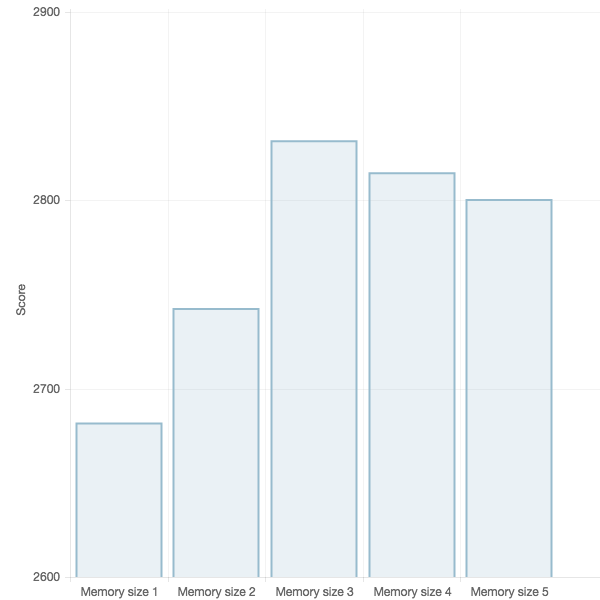
\includegraphics[scale=0.6]{figures/memsize-vs-score.png}
    \label{fig1}
\end{figure}

\subsection{Initial Population}
The initial population was a pool of prisoners having completely randomized
strategy vectors.  The population size was variable, and the effects of varying
sizes are explained in \textit{\hyperref[vpg]{section 3.7}}

\subsection{Fitness Function}

Three different fitness functions were used to evaluate a prisoners performance.
A description of each as well as performance comparisons follow.

\subsubsection{Score Against Diverse Opponents}
The prisoner being evaluated would play 100 rounds against a selection of 9
strategies which were thought to be a uniform representation of all possible
strategies.  Total score was calculated and used as a performance grade.
The nine strategies were:
\begin{enumerate}
    \item All C - Always cooperate
    \item All D - Always defect
    \item Tit for Tat - Cooperate first move, mirror opponents last move thereafter
    \item Suspicious Tit for Tat - Defect first move, mirror opponents last move
        thereafter
    \item Tit for 2 Tat - Cooperate first two moves, only cooperate if the
        opponent did not defect twice in a row thereafter
    \item Suspicious Tit for 2 Tat - Defect first two moves, only cooperate if the
        opponent did not defect twice in a row thereafter
    \item Grudger - Cooperate until the opponent defects, then defect without mercy
    \item Sucker - Defect until the opponent cooperates, then cooperate foolishly
    \item Hesitant - Only cooperate if the opponent has cooperated twice in a row
\end{enumerate}

From a shallow point of view this method of evaluating fitness was mostly
successful.  After some contemplation it was decided that the
9 strategies used were slightly biased towards those which tend to cooperate.
This left some of the prisoners produced vulnerable to rouge defectors,
and thus sub-optimal.

\subsubsection{Hamming Distance From TFT Genome}
The prisoner would be evaluated based on the hamming distance
\footnote
{\href{https://en.wikipedia.org/wiki/Hamming distance}{Hamming distance}}
between its current strategy vector and the strategy vector representing
the TFT genome.  This obviously had a tendency to produce prisoners which
acted increasingly similar to TFT.  Although the performance of said bots
was sound, this method did not produce any extraordinary or new strategies.

\subsubsection{Score Against TFT}
\label{tft}

The prisoner would be evaluated based on its score after 100 rounds against
TFT.  Since TFT is widely accepted as one of the best overall strategies it was
decided that performance against it would be a suitable benchmark.
This method seemed to produce the best results with the least
amount of computation time.  The prisoners produced behaved somewhat similarly
to TFT but contained some genome sections which differed considerably.  The result
is a prisoner which \textit{mostly} contains the desired qualities from TFT
but also includes some routines which give it an advantage in certain situations.


\subsubsection{Fitness Function Comparison}

\begin{figure}[h]
    \label{fig2}
    \caption{Graph of fitness function vs average score over 100 games}
    \centering
    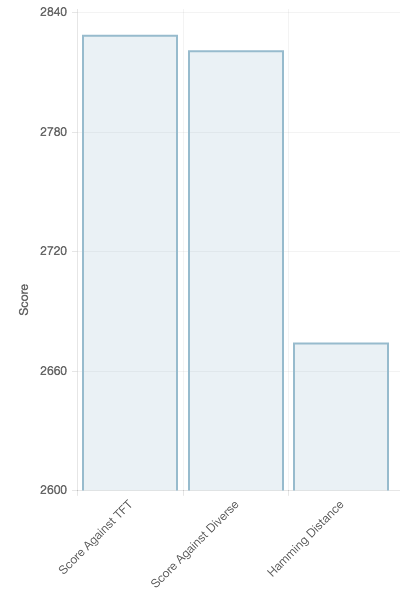
\includegraphics[scale=0.5]{figures/fit_score.png}
    \label{fig1}
\end{figure}

As evidenced by \hyperref[fig2]{figure 2} Score against TFT and Score Against Diverse
produce very similar average scores (within 10 points).  The main difference
between the two is that Score Against Diverse takes significantly longer to compute
as it is pitting the prisoner against 9 others compared to just one by Score against TFT.
For these two reasons Score against TFT is clearly the superior fitness function.

\subsection{Selection}

After evaluating fitness (explained in the previous section) a pool of
prisoners were selected to survive into the next generation.  This pool was
selected using weighted random sampling.  In order to accomplish this the
discrete cumulative density function
\footnote{\href{https://en.wikipedia.org/wiki/Cumulative distribution function}{CDF}}
, in this case an array of the cumulative sums of each prisoner's fitness value,
was calculated.  A random integer was then calculated as $p = Rand \in [0, CDF_n]$,
and binary such was performed to find the first element in the cumulative CDF array that
was greater than or equal to $p$.  The prisoner corresponding to this element
is then added to the next generation.  This process is repeated $popSize$ times
and the next generation is formed. \\

This selection method was modeled after Roulette-wheel selection via stochastic acceptance
\footnote{\href{http://arxiv.org/pdf/1109.3627.pdf}{Roulette-wheel selection}}
but has been optimized for practical usage by reducing time and space complexities.

\subsection{Cross Over}

The cross over process is trivially implemented.  Given two genomes $G_1, G_2$,
a random integer $c = Rand \in [0, min(length(G_1), length(G_2))]$ is generated
to be used as the cross over point.  Two new genomes are then given as:\\

$G'_1 = {G_1}_{[0,c)}{G_2}_{[c, length(G_2)]}$ and
$G'_2 = {G_2}_{[0, c)}{G_1}_{[c, length(G_1)]}$ \\

\begin{figure}[h]
    \caption{Crossover example for genome size 4}
    \centering
    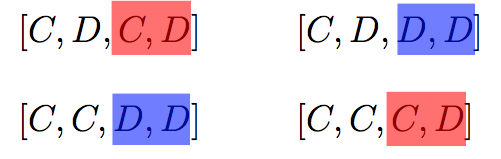
\includegraphics[scale=0.5]{figures/crossover-example.png}
\end{figure}

This cross over is applied to each adjacent pair of prisoners in the current
generation.  Since the order of the prisoners is random it follows that the pairings
are also random.

\subsection{Mutation}
\label{mutation}

The mutation phase is straightforward as well.  Each gene of the genome is changed
to a random decision $d = Rand \in [C, D]$ with a probability of $p$.  Generally
this value of $p$ is low (between 1 and 5 percent) to avoid creating unstable
evolution while still introducing some element of randomness.

\pagebreak
% stupid figure wont fit correctly without this page break

\subsection{Varying Population Size and Number of Generations}
\label{vpg}
\begin{figure}[h!]
    \caption{Blue line represents varying population, grey line varying generations}
    \centering
    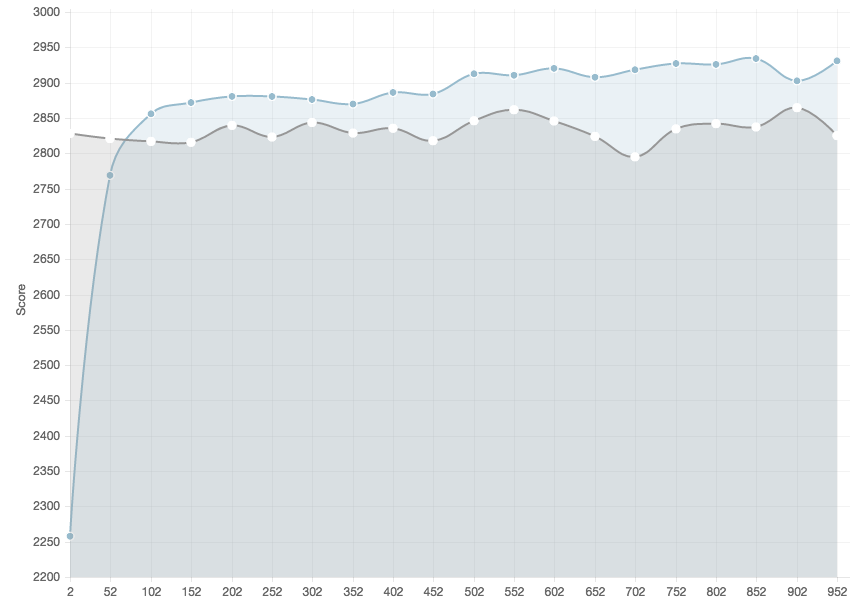
\includegraphics[scale=0.5]{figures/gen_pop_compare}
\end{figure}

An interesting thing to note is that all other factors remaining constant,
varying population size has a greater effect on score than varying the number
of generations in the evolution. As seen in the graph above, increasing the number
of generations has almost no effect on score while increasing the population
size shows a clear upward trend.  We believe this phenomenon shows that the genome
strings converge rather quickly.  Increasing population size diversifies
the gene pool and gives a more optimal convergence point, whereas increasing
the number of generations simply moves along the asymptote non productively.

\section{Hill Climbing}

The hill-climbing approach was able to recycle most of the same techniques that
were used in the genetic algorithm. The prisoners have their strategy
represented as a vector of size $4^n$, and iterative hill-climbing was used
to improve upon an initial strategy.

\subsection {Fitness Function}

As the \textit{\hyperref[tft]{Score Against TFT}} proved to be the most simple
and effective fitness function for usage in the genetic algorithm, it was
chosen for use in the hill-climbing algorithms as well.

\subsection {Successor Function}

One of the problems with developing a successor function for the IPD is that
there does not seem to be any "natural successor" for any given state (i.e
there is no natural connection from one state to another). As such, successors
must be generated randomly.\\

For this reason, the \textit{\hyperref[mutation]{random mutation function}}
used in the genetic algorithm was chosen as the successor function.

\subsection {Implementation}

The hill-climbing algorithm has a structure equivalent to: \\

\begin{algorithm}[H]
 \KwInput{Prisoner init, Rounds rounds, Mutation Rate rate}
 \KwOutput{A new improved prisoner}
 \For{$i\leftarrow 1$ \KwTo $rounds$}{
  $succ$ $\leftarrow$ mutate($init$, $rate$)\;
  \If{fitness($succ$) > fitness({$init$})}{
   $init$ $\leftarrow$ $succ$\;
  }
 }
 \KwRet{$succ$}
\end{algorithm}

Due to the fact that there is no natural connection between any given states,
the possibility of becoming stuck on a local maxima is eliminated. Rather than
gradually increasing performance along a local curve, the successors are
generated from everywhere on the curve. This allows for a simplistic algorithm
that removes the necessity of random restarts.

\section{Conclusion}

\subsection{Traits of Good Genomes}
Through a large amount of tests, it was found that the most successful genomes
had a bias towards cooperating with other prisoners. Most notably, almost all of
the successful prisoners generated would cooperate on their first move.

Rather than immediately responding to the most recent moves, the prisoners would
typically alternate in small bursts between cooperating and defecting. A consistent
pattern between the lengths of these intervals could not be found.

\subsection{Genetic Algorithm vs Hill-Climbing}
The genetic algorthm was able to consitently produce prisoners who performed
optimally against other generated and predefined strategies. This was not the
case however for the prisoners generated by hill-climbing. Most prisoners
that were created with this method found themselves in the middle of the pack,
rather than being a clear winner.

Even after greatly increasing the number of iterations to perform, prisoners
produced via hill-climbing still underperformed.

The genetic algorithm had both a greater performance floor and ceiling in comparison
to hill-climbing. The best prisoners that were produced with the genetic algorithm
scored considerably higher than that of hill-climbing, and even the worst
prisoners created genetically were dominant over the best prisoners resulting from
hill-climbing.

The reason that hill-climbing performs so poorly is that the IPD is not a problem
that is well-suited to the algorithm. Since there is no natural successor to a given state, it
is impossible to generate a neighbour that preserves locality. Additionally,
the IPD is a problem that does not have any final solution, as such there is no clear
goal to be reached.

\pagebreak

\section{Source Code}
All source code for this study was written in C++ and is
available on
\href{https://github.com/Quinny/IteratedPrisoners}{Github}

\end{document}
